\section{The Open and Closed Universes}

\paragraph{Sacred Magic}

Letter III on the \emph{Empress} is about Sacred magic, which is putting mystical revelation into practice. This requires preparation:

\begin{itemize}
\item \textbf{Mysticism}: Real contact with the Divine 
\item \textbf{Gnosis}: Taking this contact into consciousness 
\item \textbf{Magic}: Executing what mystical revelation has made known 
\end{itemize}
Unlike sacred magic, personal magic, i.e., in which the magician decides himself when and how to put esoteric teachings into practice, has certain dangers, including physical problems as well as emotional. I knew a woman, quite closely in fact, who got involved with Enochian magic. Despite her esoteric training she was anxious, emotional, inconstant, and paranoid. I don't know which came first, but at the very least the magical practice did not help her. Sacred magic offers healing, not harm.

\begin{wrapfigure}{rt}{.15\textwidth}
 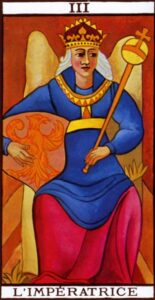
\includegraphics[scale=3]{a20221030TheOpenandClosedUniverses-img001.jpg} 
\end{wrapfigure}

Moreover, psychological and physical effects should not be pursued for their own sake. True mysticism is beyond such states, reaching something much higher. Rather, the focus needs to be on uniting the human will with God's will. The latter has been revealed to us, at least in a general way. In addition, he has a plan for your own particular life, you need to discern it.

The fruit of this union is concentrated in the blood. This is the \textbf{Holy Grail}. Power starts with divine and human sincerity, united in human words and actions. True sincerity is not cerebral, but rather it must flow in one's life blood. We read:

\begin{quotex}
The more sincerity there is in the human word or action, the more there is the vital essence of blood. When it happens —and the Angels fall down in adoration when this occurs — that the human wish is in accord with the divine, the Holy Blood is then united to the vital essence of the human blood and the Mystery of the God-Man is repeated, and also the miraculous power of the God-Man is reiterated. Here is the power of sacred magic — or its sceptre. 

\end{quotex}
The aims of sacred magic are:

\begin{itemize}
\item The freedom to see (give sight to the blind) 
\item The freedom to hear (hearing to the deaf) 
\item The freedom to walk (the ability to walk to the lame) 
\item The freedom to live (life to the dead) 
\item The freedom to follow an ideal (good news to the poor) 
\item The freedom to be truly oneself (casting out evil spirits from the possessed) 
\end{itemize}
In sum, it is the restoration of freedom, particularly from doubt, fear, hate, apathy, and despair.

The fallen angels (e.g., Satan, Belial, Lucifer, Mephistopheles) never deprive anyone of his freedom, and their only weapon is Temptation. However, possession has nothing to do with temptation. That is because human perversity is capable of much worse evil. The human mind will engender elemental beings and subsequently becomes the slave of its own creation.

\paragraph{Selection and Election}

Letter X on the \emph{Wheel of Fortune} mentions that there are two ways of looking at the world:

\begin{itemize}
\item \textbf{exoterically}, as a mechanical process or 
\item \textbf{esoterically}, as a cosmic drama comprising the Fall, perdition, redemption, and salvation 
\end{itemize}
The analogy of a passenger ship illustrates these views:

\begin{itemize}
\item The passengers buy a ticket and are passive. For them, the ship is an automatic process leading them to their destination 
\item The crew, on the other hand, are involved in the drama of keeping the ship on course via work, watches, maneuvering, and orientation. 
\end{itemize}

\begin{wrapfigure}{rt}{.15\textwidth}
 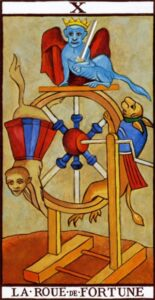
\includegraphics[scale=3]{a20221030TheOpenandClosedUniverses-img002.jpg} 
\end{wrapfigure}

Analogously, evolution can be understood in two ways.

\begin{itemize}
\item It can be seen as a ``natural process" through the eyes of the passengers 
\item It is a ``tragedy and drama" as the crew experiences it. 
\end{itemize}
The passengers are ready to believe in determinism, fatalism, or naturalism. This offloads responsibility to Nature, God, the stars, i.e., anywhere except the moral human being. Of course, the passengers can point out the evidence for natural evolution, and they are not mistaken as far as it goes. But the esoterist looks for the moral cause:

\textbf{Joseph de Maistre} was not interested in the logic of facts, since, as he asserted, the Law of Gravity does not cause the rock to fall. Instead, he was concerned with the moral logic, or the moral cause of events. Science deals with facts yet can never answer the question, ``Why?" Ultimately, therefore, it comes down to the moral will, which is the real cause. And an evil will brings about evil effects

Hence, while the exoteric explanation sees ``natural selection" as the agent effecting change, the esoteric explanation sees ``election". One is chosen to be on the crew, to participate in the cosmic drama as an active agent.

\paragraph{The Two Wheels}
In the drama of Creation, God created in six days and rested on the seventh. This is presented by a circle with the seventh day at the top. However, as a day of rest, it is open, so the circle is not closed: there is an opening.

The serpent, on the other hand, bites his tail, creating a closed circle. This is the ouroboros. The serpent world is endless repetition, cycle after cycle, the eternal return. Buddha, Solomon, and Nietzsche sensed this. The Buddha looked for an escape, Solomon despaired, But Nietzsche praised it.

There are no miracles in the closed world of the Serpent, just the same thing over and over, following an impersonal cosmic process. This applies also to the doctrine of cosmic cycles in some Eastern and New Age teachings.

True religion shows the open world, in which miracles are possible. Natural processes do not explain the totality of the universe. That is the ``good news": the world is not an eternal prison, there is an entrance and an exit.

The Fall is the cosmic event set in motion by the closed circle of the serpent biting his tail, locking those inside the world. Hence, Redemption is the cosmic act of the Reintegration of the Fallen world in stages:

\begin{enumerate}
\item An opening in the closed circle is created (religion, initiation, prophecy) 
\item A exit path is taught (Buddha) 
\item Avatars enter through this door 
\item The fallen world is transformed from within by the radiation of the incarnated Word (Jesus Christ) 
\end{enumerate}


\flrightit{Posted on 2022-10-30 by Cologero }
